% !TEX root = ../main.tex
\chapter{Background}
\label{Background}

\section*{Electricity as a Common Pool Resource}
A Common Pool Resource is a depletable resource which can be utilised by a group of people, characterised by a reduction in the availability of this resource as individuals withdraw or utilise this resource \cite{Ostrom:90}.  Electricity can be a Common Pool Resource if there exists a finite amount of electricity generation capacity. As users connect demand appliances to the generators, the availability of electricity supply for additional demand diminishes.

In developing communities with significant generation from renewable sources such as wind and solar, the availability of power is subject to variation between periods in time. This inherent volatility in the amount of available resource could increase the likelihood of selfish actions of by individuals in the community.

Common Property Regimes can be formed to maintain the Common Pool Resources by controlling the access to the resource. 

\section*{Decentralised Community Energy Systems as a Holonic System} %CITE PITT HERE
A holonic system (or holarchy) is a system which is composed of interrelated subsystems or institution, each of which are in turn composed of sub-subsystems  or institution and so on, recursively until reaching a lowest level of "elementary" subsystems. Each system, sub-system or institution has a well-defined set of goals or objectives which is achieved through enforcing a set of rules on its members (subsystems, sub-institutions and elementary entities).\pdfmarkupcomment[markup=Highlight,color=yellow]{[[[[[[ "CITE PITT HERE" ]]]]]]]}{Highlight} It is this type of Common Property Regime that will be explored in this project to maintain the Common Pool Resource that is electricity. 


In the context of a rural Decentralised Community Energy system, a network between households, communities and even villages to pool and share electricity as a common pool resource can be modelled as a holonic system. The holonic system in this case would be composed of communities such as Districts, Provinces, Sectors which are composed of sub-communities such as Towns and Villages. The sub-communities would be composed of many "elementary" such as households, businesses and other points of connection for electricity. Each community or institution has the goal of fairly allocating electricity to all members. This goal would be achieved with the assumption that they are provided with the necessary infrastructure and powers for enforcing quotas and contribute to a common pool of electricity.


\section*{Rural Communities in Rwanda}
With an estimated 25\% rural electrification rate in 2009 \cite{IEA-web:2015}, rural Africa is one obvious candidate for simulation scenarios. Vast amounts of rural communities remain un-electrified. For a realistic simulation scenario, knowledge of existing infrastructure in place will need to be obtained. With many areas within many countries in Africa, Rwanda in particular has been identified as a good potential simulation scenario to research. Data is difficult to source for rural communities in developing countries, however in the case of Rwanda, some data can be easily from the student society e.quinox. e.quinox is a student-led society which aims to find a scalable solution for rural electrification who mainly operate in Rwanda \cite{e.quinox-web:2015}. The subsections below outline some of the ways remote rural communities are able to access electricity in Rwanda.

\subsection*{Electricity Generation}
One of the solutions currently being implemented by e.quinox is the "Energy Kisok" model \cite{e.quinox-EK-web:2015}. The "Energy Kiosk" model features an Energy Kiosk - a building where the generation, storage and distribution of electricity takes place.
In e.quinox operated kiosks, electricity is generated from renewable sources.
Traditionally, this has been with solar panels. However, hydro-electric generation has been demonstrated to be feasible with the recent construction of a "Hydro Kiosk" at Rugaragara Falls in Southern Rwanda.

\subsection*{Storage and Distribution}
Within each kiosk, electricity that is generated is stored in storage batteries placed in the kiosks. The storage batteries regulate power output and allows access to electricity in the kiosk even during periods of no electricity generation.

\subsubsection*{Battery Box}
In the absence of any electricity distribution infrastructure, e.quinox has traditionally provided a number of portable batteries for the purpose of electricity distribution. An example of the portable batteries can be seen in Figure \ref{fig:AmaziBox}.

\begin{figure}[h!]
\centering
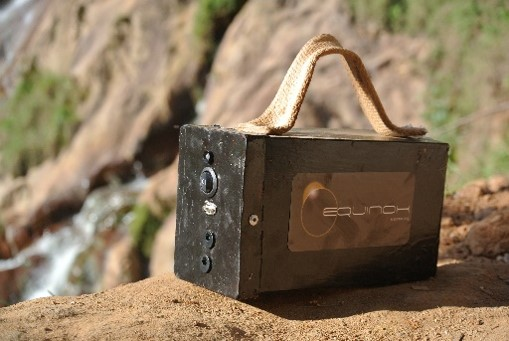
\includegraphics[scale=0.7]{Images/AmaziBox.jpg}
\caption{First Generation e.quinox Battery Boxes deployed at Rugaragara Falls Kiosk}
\label{fig:AmaziBox}
\end{figure}



Consumers from local community pay to hire the battery boxes under one of two payment schemes: pay-per-recharge and pay-per-month \cite{e.quinox-Hydro-web:2012}. The biggest difference between the two schemes are that users can recharge as often as they would like with pay-per-month. Both payment schemes involve the recharge of the boxes at the energy kiosk when they are depleted of energy.

A potential use case of this project can be the simulation of charging of battery boxes at an energy kiosk. This could alleviate congestion and improve asset utilisation of the existing distribution systems by reducing the turn-around time of battery boxes for customers.

\subsubsection*{Micro Grid}
With the recent completion of a hydro-electric kiosk. e.quinox for the first time has a kiosk with access to an always-on generator. With a limited number of battery boxes in circulation and a constant generation available during the off-peak hours, there is excess capacity for electricity generation.

To improve utilisation of the generator in the kiosk, e.quinox has recently started conducting a feasibility study into constructing a transmission line and a distribution network which will serve a village near the kiosk with a view to make the most of the electricity generated.

Preliminary surveys conducted in the nearest village to the kiosk indicates the demand could exceed the amount of excess power generated by the kiosk. 

The result of this project can be used in conjunction with e.quinox to conduct the feasibility study of implementing the Micro-Grid. Should a trading platform for energy also be built, the Micro-Grid could serve as a test-bed for this new system.

\subsubsection*{Standalone Solution}
The Standalone Solution is an independent electrification solution which was recently developed by e.quinox for customers who live far from energy kiosks.

The Stand-alone solution consists of a pay-as-you-go solar electricity generation and storage kit, known as the Izuba.Box \cite{e.quinox-Standalone-web:2012}.  With the Izuba.Box, customers no longer have to travel regularly back to the Energy Kiosk for electricity. Solar panels are installed on the customer’s roof, and is connected to a sealed box which contains a large battery box. The attached large battery box allows a regulated power output and access to electricity during dark hours. 

With the customers not returning to Energy Kiosks, the battery boxes are not hired out like the battery boxes are. The high capital costs of the independent solar system is spread over typically a two year rent-to-own payment plan using a mobile payment system.

It is hoped that the Standalone Solution and additional generation from the Energy Kiosk can be complemented the battery boxes in circulation to provide a continuous access to electricity to all households in the village.

\begin{figure}[h!]
\centering
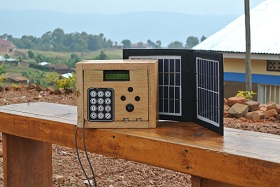
\includegraphics[scale=3]{Images/standalone_box.jpg}
\caption{First Generation Izuba.Box deplyed in Minazi, Northern Rwanda}
\label{fig:IzubaBox}
\end{figure}

\subsection*{In the context of the Project}
In developing countries such as Rwanda, poor communities with no access to grid electricity are often in isolated locations. In these areas, fuel for generators are often difficult to obtain. Other available sources of electricity such as solar and wind power are highly dependent other variables such as weather. It is also highly unlikely that they will have access to redundancies to ensure continual access much like the electricity we receive from the national distribution and transmission network in the UK. It is therefore beneficial for systems such as the one we are modelling as it has lower barriers to entry than access to 

% \subsection{Additional Research}
% e.quinox in Rwanda only presents us with one scenario. Additional research is required for other regions such as South America and the Indian Subcontinent to look at potential new scenarios and use cases for various generators and electrical appliances.

% The information above only outlines the existing infrastructures in place. Additional work needs to be done to obtain relevant usage data from e.quinox customers and other electricity users to accurately build a relevant generation mix and demand model.

% In some regions such as Minazi, e.quinox provides the only source of accessible electricity for the local populace. Data on their usage should be more readily available than some of the other locations in other countries. 